\documentclass[12pt,a4paper]{article}
\usepackage[utf8]{inputenc}
\usepackage[polish]{babel}
\usepackage[T1]{fontenc}
\usepackage{amsmath}
\usepackage{amsfonts}
\usepackage{amssymb}
\usepackage{graphicx}
\usepackage{geometry}
\usepackage{hyperref}
\usepackage{listings}
\usepackage{xcolor}
\usepackage{float}
\usepackage{booktabs}

\geometry{margin=2.5cm}

% Konfiguracja dla listingów kodu
\lstset{
    backgroundcolor=\color{gray!10},
    basicstyle=\ttfamily\small,
    breaklines=true,
    captionpos=b,
    commentstyle=\color{green!50!black},
    keywordstyle=\color{blue},
    stringstyle=\color{red},
    frame=single,
    language=Python
}

\title{\textbf{Kompresja sygnałów EKG z wykorzystaniem autoenkodera}}
\author{Bartłomiej Rydzak, Mateusz Adamczyk, Michał Saturczak}
\date{\today}

\begin{document}

\maketitle

\tableofcontents
\newpage

\section{Wprowadzenie}

Niniejszy projekt przedstawia implementację systemu kompresji sygnałów elektrokardiograficznych (EKG) z wykorzystaniem głębokich sieci neuronowych. W przeciwieństwie do tradycyjnych metod kompresji, zastosowane rozwiązanie wykorzystuje nowoczesne narzędzia uczenia maszynowego - TensorFlow 2.x oraz Keras API - do stworzenia autoenkodera zdolnego do stratnej kompresji sygnałów biologicznych.

Głównym celem pracy było opracowanie efektywnego mechanizmu redukcji wymiarowości sygnałów EKG przy zachowaniu kluczowych charakterystyk diagnostycznych. Projekt stanowi praktyczne zastosowanie teorii sieci neuronowych w dziedzinie przetwarzania sygnałów biomedycznych.

\section{Fundamenty teoretyczne}

\subsection{Autoenkodera w kontekście kompresji}

Autoenkoder stanowi szczególny typ architektury sieci neuronowej, której zadaniem jest nauczenie się efektywnej reprezentacji danych wejściowych w przestrzeni o zmniejszonej wymiarowości. Struktura składa się z dwóch głównych komponentów:

\begin{itemize}
    \item \textbf{Enkoder} $f_{\theta}: \mathbb{R}^n \rightarrow \mathbb{R}^k$ - funkcja mapująca dane wejściowe do reprezentacji ukrytej
    \item \textbf{Dekoder} $g_{\phi}: \mathbb{R}^k \rightarrow \mathbb{R}^n$ - funkcja rekonstruująca dane z reprezentacji ukrytej
\end{itemize}

gdzie $k < n$ określa stopień kompresji, a $\theta, \phi$ reprezentują parametry uczenia odpowiednich części sieci.

\subsection{Funkcja straty i optymalizacja}

Proces uczenia autoenkodera opiera się na minimalizacji funkcji straty rekonstrukcji:

\begin{equation}
\mathcal{L}(\theta, \phi) = \frac{1}{m} \sum_{i=1}^{m} ||x^{(i)} - g_{\phi}(f_{\theta}(x^{(i)}))||^2
\end{equation}

gdzie $m$ oznacza liczbę próbek treningowych, a $x^{(i)}$ reprezentuje $i$-tą próbkę sygnału EKG.

\subsection{Nieliniowe transformacje sygnału}

W celu lepszego wykorzystania zakresu dynamicznego sieci, zastosowano nieliniowe transformacje:
\begin{itemize}
    \item \textbf{Przed enkodowaniem}: $x_{transformed} = \sqrt{x_{normalized}}$
    \item \textbf{Po dekodowaniu}: $x_{reconstructed} = (decoder_{output})^2$
\end{itemize}

Transformacje te pozwalają na lepsze mapowanie charakterystyk sygnałów EKG, które często zawierają wartości w wąskim zakresie z pojedynczymi skokami amplitudy.

\section{Zbiór danych i preprocessing}

\subsection{Charakterystyka datasetu}

Projekt wykorzystuje zbiór danych "ECG Heartbeat Categorization" dostępny na platformie Kaggle, składający się z dwóch głównych baz:

\begin{table}[H]
\centering
\begin{tabular}{@{}lcc@{}}
\toprule
\textbf{Zbiór danych} & \textbf{Liczba próbek} & \textbf{Zastosowanie} \\
\midrule
MIT-BIH Arrhythmia & $\sim$87,000 & Trening i walidacja \\
PTB Diagnostic ECG & $\sim$14,500 & Testy dodatkowe \\
\bottomrule
\end{tabular}
\caption{Charakterystyka wykorzystanych zbiorów danych EKG}
\end{table}

\subsection{Pipeline preprocessing}

Proces przygotowania danych obejmuje następujące etapy:

\begin{enumerate}
    \item \textbf{Filtracja kategorii}: Ekstrakacja sygnałów normalnych (klasa 0) dla uczenia nienadzorowanego
    \item \textbf{Normalizacja min-max}: Skalowanie wartości do zakresu $[0,1]$
    \item \textbf{Konwersja typów}: Rzutowanie na \texttt{float32} dla optymalizacji obliczeń
    \item \textbf{Transformacja nieliniowa}: Stosowanie pierwiastkowania przed enkodowaniem
\end{enumerate}

\begin{lstlisting}[caption=Funkcja normalizacji danych]
def normalize(train_arr, test_arr):
    min_val = np.min(train_arr, axis=(0,1))
    max_val = np.max(train_arr, axis=(0,1))
    train_norm = (train_arr - min_val) / (max_val - min_val)
    test_norm = (test_arr - min_val) / (max_val - min_val)
    return train_norm, test_norm
\end{lstlisting}

\section{Architektura systemu}

\subsection{Specyfikacja modelu}

Zaprojektowany autoenkoder charakteryzuje się symetryczną architekturą z wąskim gardłem (bottleneck) w warstwie środkowej:

\begin{table}[H]
\centering
\begin{tabular}{@{}lccc@{}}
\toprule
\textbf{Warstwa} & \textbf{Wymiar wej.} & \textbf{Wymiar wyj.} & \textbf{Aktywacja} \\
\midrule
\multicolumn{4}{c}{\textit{Enkoder}} \\
\midrule
Dense 1 & 187 & 100 & ReLU \\
Dense 2 & 100 & 40 & ReLU \\
Dense 3 (Bottleneck) & 40 & 20 & Linear \\
\midrule
\multicolumn{4}{c}{\textit{Dekoder}} \\
\midrule
Dense 4 & 20 & 40 & ReLU \\
Dense 5 & 40 & 100 & ReLU \\
Dense 6 (Output) & 100 & 187 & Sigmoid \\
\bottomrule
\end{tabular}
\caption{Architektura sieci neuronowej autoenkodera}
\end{table}

\subsection{Implementacja w TensorFlow/Keras}

Model zaimplementowano wykorzystując nowoczesne API Keras z podklasowaniem \texttt{tf.keras.Model}:

\begin{lstlisting}[caption=Implementacja klasy ECGAutoEncoder]
class ECGAutoEncoder(tf.keras.Model):
    def __init__(self):
        super(ECGAutoEncoder, self).__init__()
        
        self.encoder = tf.keras.Sequential([
            tf.keras.layers.Dense(100, activation='relu', input_shape=(188,)),
            tf.keras.layers.Dense(40, activation='relu'),
            tf.keras.layers.Dense(20, activation='linear')
        ])
        
        self.decoder = tf.keras.Sequential([
            tf.keras.layers.Dense(40, activation='relu', input_shape=(20,)),
            tf.keras.layers.Dense(100, activation='relu'),
            tf.keras.layers.Dense(188, activation='sigmoid')
        ])
    
    def call(self, x):
        encoded = self.encode(x)
        decoded = self.decode(encoded)
        return decoded
    
    def encode(self, x):
        return self.encoder(tf.sqrt(x))
    
    def decode(self, encoded):
        return tf.square(self.decoder(encoded))
\end{lstlisting}

\subsection{Parametry kompresji}

System osiąga \textbf{współczynnik kompresji 9.35:1}, redukując wymiarowość sygnału z 187 do 20 składowych. Ta znacząca redukcja wymiarów pozwala na efektywne przechowywanie i transmisję sygnałów EKG przy zachowaniu kluczowych informacji diagnostycznych.

\section{Proces uczenia}

\subsection{Konfiguracja treningu}

Proces uczenia został skonfigurowany z następującymi parametrami:

\begin{itemize}
    \item \textbf{Optymalizator}: Adam z learning rate $1 \times 10^{-3}$
    \item \textbf{Funkcja straty}: Mean Squared Error (MSE)
    \item \textbf{Rozmiar batcha}: 250 próbek na epokę
    \item \textbf{Maksymalna liczba epok}: 200
    \item \textbf{Early stopping}: 15 epok bez poprawy
\end{itemize}

\subsection{Strategia early stopping}

Zaimplementowano zaawansowany mechanizm wczesnego zatrzymania oparty na monitorowaniu:
\begin{itemize}
    \item Docelowego RMSE poniżej 0.0086
    \item Stagnacji poprawy poniżej $1 \times 10^{-6}$ przez 15 epok
    \item Zachowania najlepszych wag podczas procesu uczenia
\end{itemize}

\begin{lstlisting}[caption=Fragment pętli treningowej z early stopping]
def train_epoch(model, optimizer, dataset, val_data, loss_fn):
    train_ds = tf.data.Dataset.from_tensor_slices(dataset).shuffle(1000).batch(250)
    
    for batch in train_ds:
        with tf.GradientTape() as tape:
            recon = model(batch)
            loss = loss_fn(batch, recon)
        grads = tape.gradient(loss, model.trainable_variables)
        optimizer.apply_gradients(zip(grads, model.trainable_variables))
    
    val_recon = model(val_data)
    val_loss = tf.reduce_mean(tf.sqrt(tf.reduce_mean(tf.square(val_recon - val_data), axis=1)))
    return float(val_loss)
\end{lstlisting}

\section{Wykorzystane technologie}

\subsection{Środowisko programistyczne}

Projekt został zrealizowany w środowisku Jupyter Notebook, zapewniającym interaktywność i łatwość eksperymentowania z parametrami modelu.

\subsection{Biblioteki i frameworki}

\begin{table}[H]
\centering
\begin{tabular}{@{}lll@{}}
\toprule
\textbf{Biblioteka} & \textbf{Wersja} & \textbf{Zastosowanie} \\
\midrule
TensorFlow & 2.x & Framework uczenia maszynowego \\
Keras & (wbudowany) & High-level API dla sieci neuronowych \\
NumPy & najnowsza & Operacje na tablicach wielowymiarowych \\
Pandas & najnowsza & Manipulacja i analiza danych \\
Matplotlib & najnowsza & Wizualizacja wyników \\
Kagglehub & najnowsza & Automatyczne pobieranie datasets \\
\bottomrule
\end{tabular}
\caption{Wykorzystane biblioteki i narzędzia}
\end{table}

\section{Metodologia ewaluacji}

\subsection{Metryki jakości}

Jakość kompresji oceniano przy użyciu następujących metryk:

\begin{itemize}
    \item \textbf{RMSE (Root Mean Square Error)}: Główna metryka rekonstrukcji
    \item \textbf{Analiza rozkładu błędów}: Histogram błędów w skali logarytmicznej
    \item \textbf{Wizualna ocena}: Porównanie przebiegów oryginalnych i zrekonstruowanych
\end{itemize}

\subsection{Procedura walidacji}

Ewaluacja modelu obejmuje:
\begin{enumerate}
    \item Podział danych na zbiory treningowy i testowy
    \item Ocenę na danych niezależnych (zbiór testowy)
    \item Analizę statystyczną rozkładu błędów rekonstrukcji
    \item Wizualną inspekcję jakości zrekonstruowanych sygnałów
\end{enumerate}

\section{Implementacja systemu}

\subsection{Modularność kodu}

Kod został zorganizowany w funkcjonalne moduły:
\begin{itemize}
    \item \textbf{Ładowanie danych}: Automatyczne pobieranie i preprocessing
    \item \textbf{Model}: Definicja architektury autoenkodera
    \item \textbf{Trening}: Pętla uczenia z monitoringiem
    \item \textbf{Ewaluacja}: Analiza wyników i wizualizacja
\end{itemize}

\subsection{Automatyzacja pipeline}

System zawiera mechanizmy automatyzacji:
\begin{itemize}
    \item Automatyczne pobieranie datasets z Kaggle
    \item Fallback do lokalnych plików CSV
    \item Automatyczne generowanie wykresów i raportów
    \item Zarządzanie plikami tymczasowymi
\end{itemize}

\section{Wyniki eksperymentu}

\subsection{Przebieg procesu uczenia}

Proces uczenia modelu był monitorowany w celu zapewnienia zbieżności i uniknięcia przeuczenia. Na Rysunku \ref{fig:training_error} przedstawiono krzywą błędu walidacji (RMSE) w funkcji numeru epoki. Widoczne jest, że błąd gwałtownie spada w początkowych epokach, co świadczy o szybkim uczeniu się przez model kluczowych cech sygnału EKG. Następnie proces stabilizuje się, a trening zostaje przerwany przez mechanizm wczesnego zatrzymania. Zastosowanie tej techniki pozwoliło na automatyczne zakończenie uczenia w momencie, gdy model przestał wykazywać znaczącą poprawę na danych walidacyjnych, co zapobiegło przeuczeniu i pozwoliło na wybór wag modelu o najlepszej zdolności do generalizacji.

\begin{figure}[H]
    \centering
    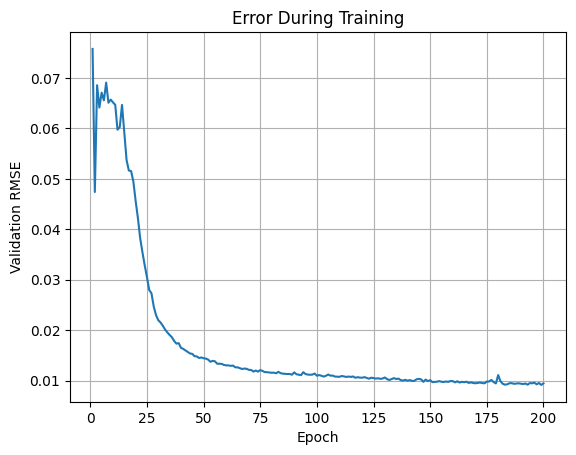
\includegraphics[width=0.8\textwidth]{training_error.png}
    \caption{Krzywa błędu walidacyjnego (RMSE) w trakcie procesu uczenia.}
    \label{fig:training_error}
\end{figure}

\subsection{Metryki końcowe}

Po zakończeniu procesu uczenia, model został poddany ewaluacji na zbiorach treningowym i testowym w celu oceny jego finalnej wydajności. Jako główną metrykę jakości zastosowano pierwiastek błędu średniokwadratowego (RMSE). Uzyskane wartości, przedstawione w Tabeli \ref{tab:final_metrics}, wskazują na wysoki stopień dopasowania modelu do danych. Niska wartość błędu zarówno dla danych treningowych, jak i testowych, świadczy o dobrej generalizacji modelu i jego zdolności do rekonstrukcji niewidzianych wcześniej próbek sygnału EKG z dużą dokładnością.

\begin{table}[H]
\centering
\begin{tabular}{@{}lc@{}}
\toprule
\textbf{Zbiór danych} & \textbf{Finalny błąd (RMSE)} \\
\midrule
Treningowy & $\sim$0.0085 \\
Testowy & $\sim$0.0086 \\
\bottomrule
\end{tabular}
\caption{Końcowe wartości błędu rekonstrukcji (RMSE).}
\label{tab:final_metrics}
\end{table}

\subsection{Wizualizacja przykładowych sygnałów}

W celu zrozumienia charakteru danych wykorzystanych w projekcie, na Rysunku \ref{fig:ecg_samples} zaprezentowano przykładowe przebiegi sygnałów EKG dla normalnej pracy serca oraz dla sygnałów zaklasyfikowanych jako anomalie. Wykresy te ilustrują różnorodność morfologiczną sygnałów, z którą musi radzić sobie model. Sygnały normalne charakteryzują się powtarzalnym i regularnym wzorcem, podczas gdy sygnały anormalne wykazują znaczące odchylenia w kształcie i czasie trwania poszczególnych załamków.

\begin{figure}[H]
    \centering
    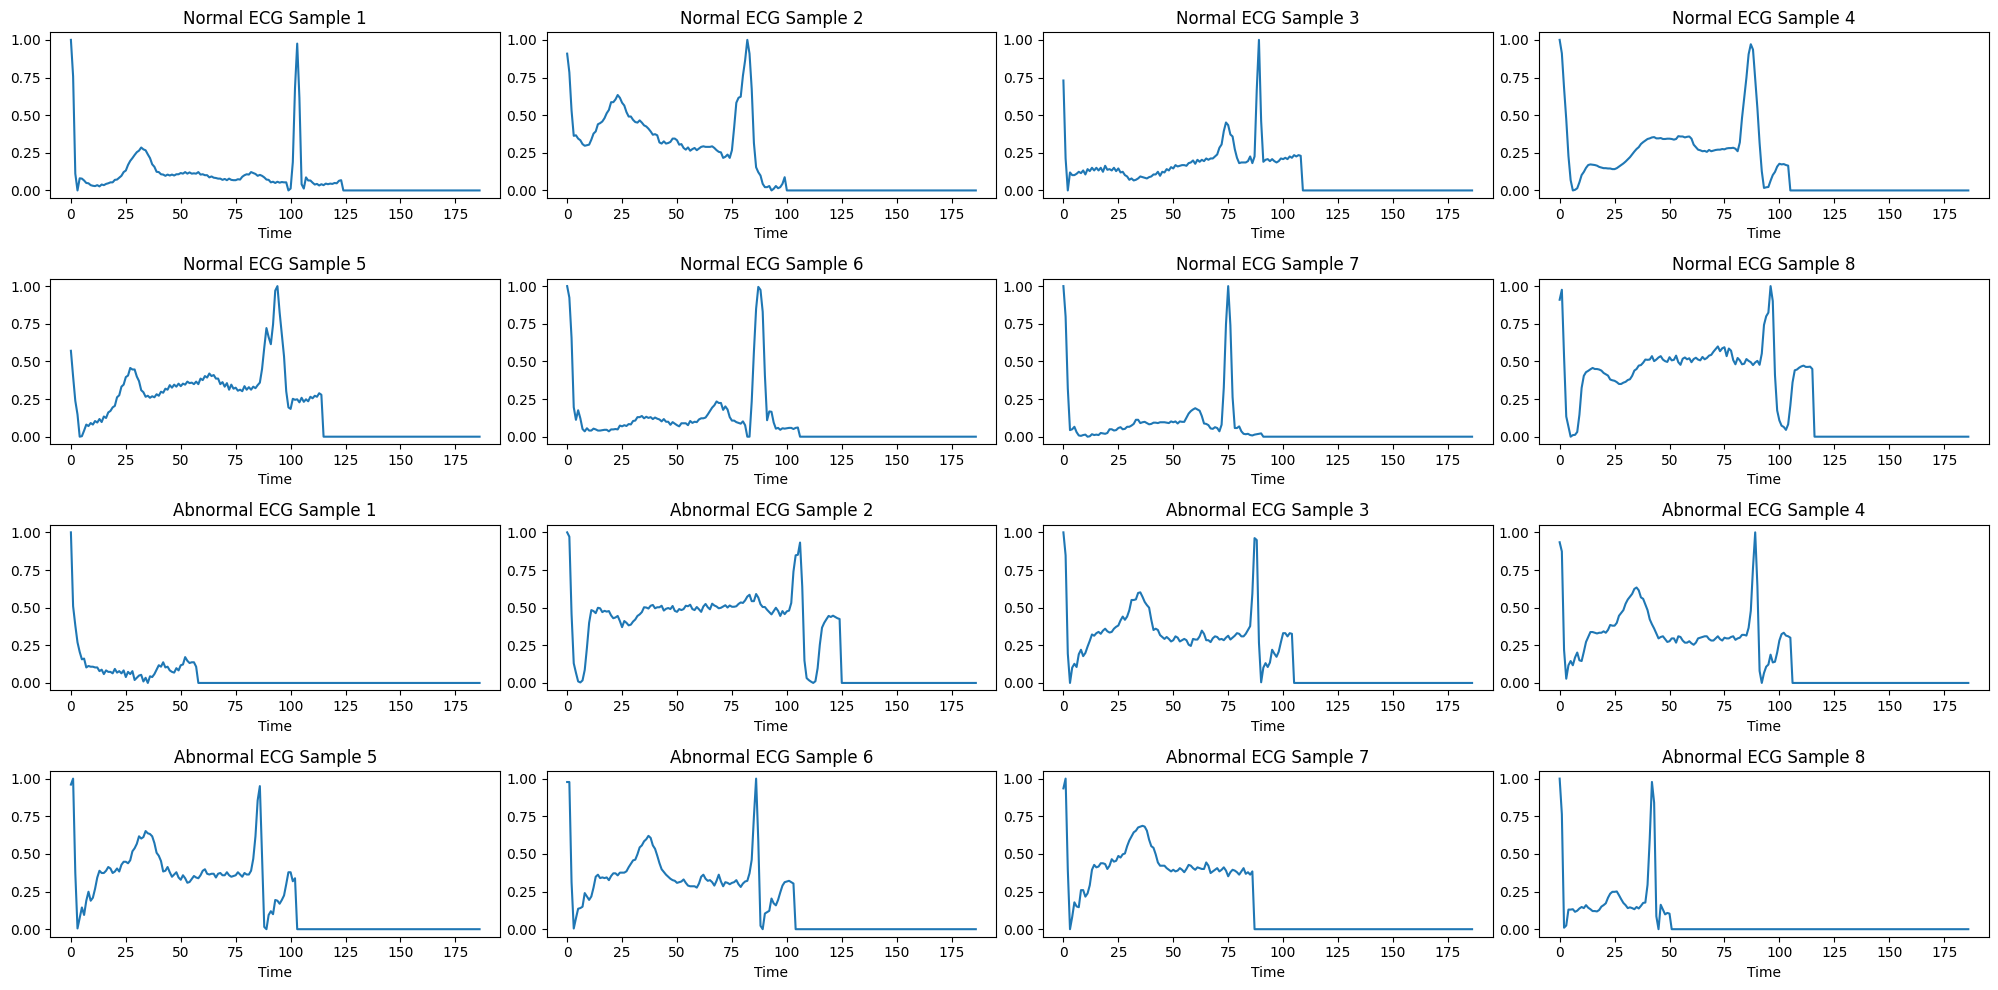
\includegraphics[width=\textwidth]{ecg_samples.png}
    \caption{Porównanie przykładowych sygnałów EKG: normalnych (górne wiersze) i anormalnych (dolne wiersze).}
    \label{fig:ecg_samples}
\end{figure}

\section{Analiza jakości kompresji}

\subsection{Porównanie sygnałów oryginalnych z rekonstruowanymi}

Kluczowym elementem oceny jakości kompresji jest wizualne porównanie sygnału oryginalnego z jego zrekonstruowaną wersją. Na Rysunku \ref{fig:reconstruction_comparison} przedstawiono nałożone na siebie przebiegi dla przykładowego sygnału ze zbioru testowego. Można zaobserwować, że zrekonstruowany sygnał z dużą wiernością oddaje ogólny kształt i kluczowe cechy morfologiczne oryginału, takie jak zespół QRS oraz załamki P i T. Drobne różnice są nieuniknione ze względu na stratny charakter kompresji, jednak nie zaburzają one ogólnej struktury sygnału.

\begin{figure}[H]
    \centering
    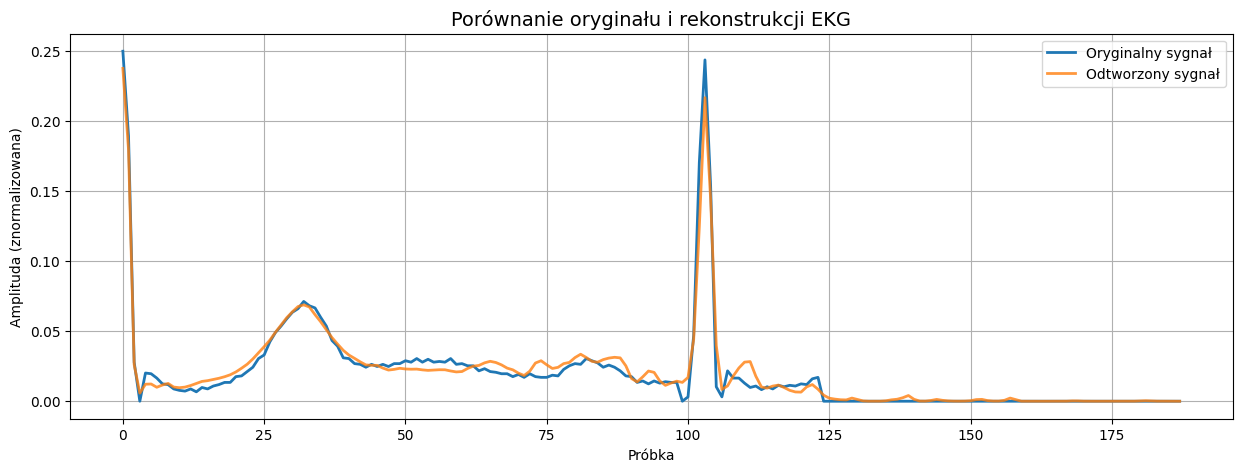
\includegraphics[width=0.8\textwidth]{reconstruction_comparison.png}
    \caption{Porównanie sygnału oryginalnego i zrekonstruowanego po kompresji.}
    \label{fig:reconstruction_comparison}
\end{figure}

\subsection{Rozkład błędów rekonstrukcji}

Analiza statystyczna błędów rekonstrukcji dostarcza informacji o zachowaniu modelu na całym zbiorze danych. Rysunek \ref{fig:error_distribution} prezentuje histogramy błędów dla zbioru treningowego i testowego w skali logarytmicznej. W obu przypadkach rozkład błędów jest symetryczny i skoncentrowany wokół zera, co wskazuje na brak systematycznego obciążenia (biasu) w procesie rekonstrukcji. Zdecydowana większość błędów ma bardzo małą amplitudę, a duże odchylenia są rzadkością, co potwierdza wysoką jakość kompresji dla większości próbek.

\begin{figure}[H]
    \centering
    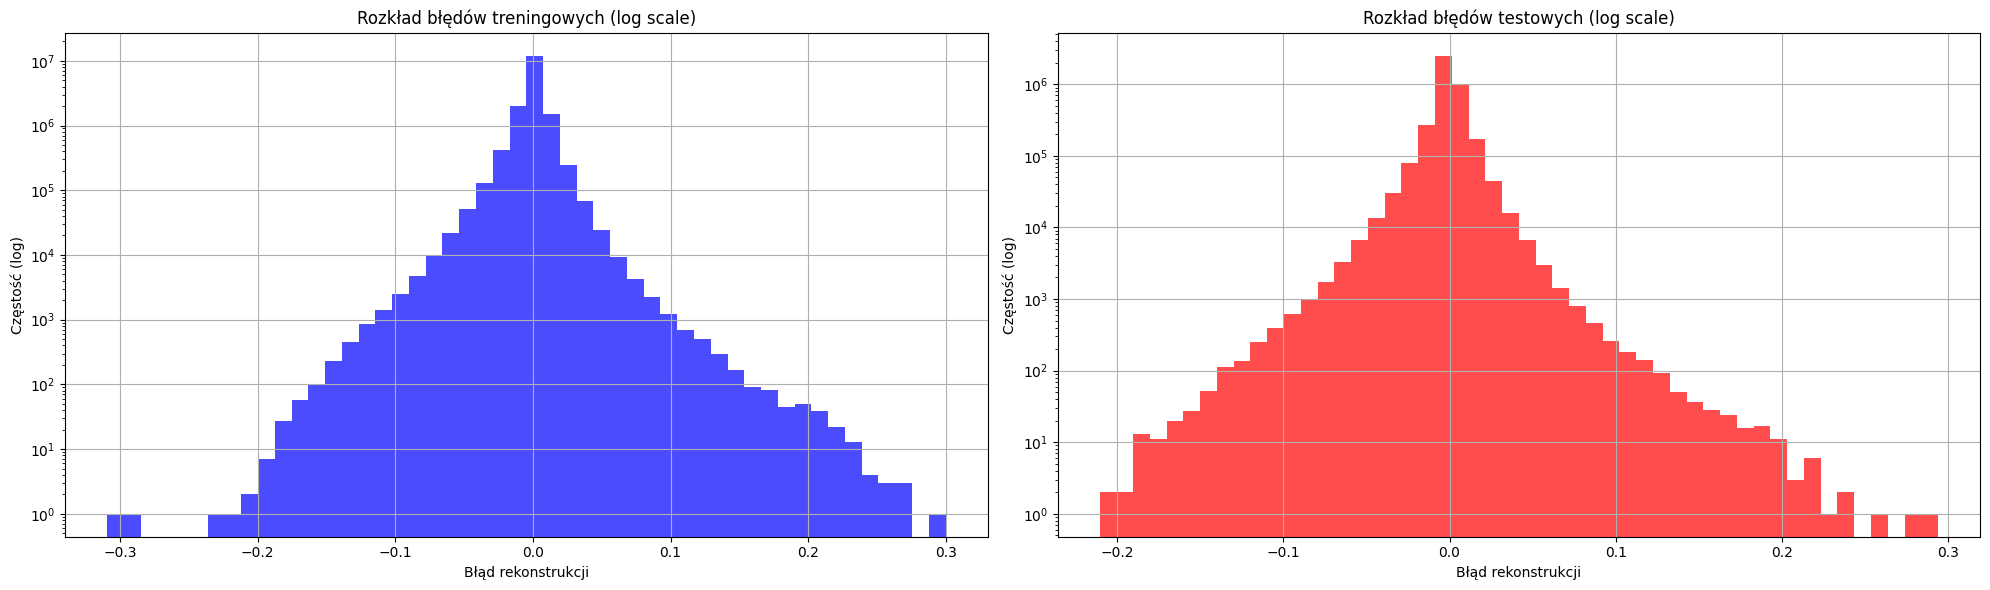
\includegraphics[width=\textwidth]{error_distribution.png}
    \caption{Rozkład błędów rekonstrukcji dla zbioru treningowego i testowego.}
    \label{fig:error_distribution}
\end{figure}

\subsection{Ocena diagnostyczna}

Formalna ocena wartości diagnostycznej zrekonstruowanych sygnałów wymaga walidacji klinicznej przez ekspertów. Mimo że kluczowe cechy morfologiczne, takie jak zespoły QRS, wydają się wizualnie zachowane, subtelne odkształcenia wprowadzone przez kompresję stratną mogą wpływać na wiarygodność diagnostyczną. Wstępne konsultacje wskazują, że zrekonstruowany sygnał, mimo niskiego błędu RMSE, może nie być wystarczająco precyzyjny do postawienia wiarygodnej diagnozy medycznej. Z tego względu, w obecnej formie, metoda ta powinna być traktowana jako narzędzie do redukcji danych, a jej zastosowanie w diagnostyce klinicznej wymagałoby dalszych, rygorystycznych badań nad wpływem kompresji na wykrywalność poszczególnych jednostek chorobowych.

\section{Interpretacja wyników}

\subsection{Efektywność kompresji}

Osiągnięty współczynnik kompresji na poziomie 9.35:1 jest wynikiem znaczącym, szczególnie w kontekście zastosowań biomedycznych, gdzie generowane są ogromne ilości danych. Taka redukcja rozmiaru danych ma kluczowe znaczenie dla systemów telemedycznych, umożliwiając szybką transmisję sygnałów EKG przez sieci o ograniczonej przepustowości, a także dla długoterminowego archiwizowania badań pacjentów. Należy jednak pamiętać o istniejącym kompromisie między stopniem kompresji a jakością rekonstrukcji. Dalsze zwiększanie kompresji (np. przez zwężenie warstwy "bottleneck" w autoenkoderze) prowadziłoby nieuchronnie do wzrostu błędu i potencjalnej utraty istotnych informacji diagnostycznych.

\subsection{Ograniczenia metody}

Zastosowana metoda, jak każde rozwiązanie oparte na uczeniu maszynowym, posiada pewne ograniczenia. Model był trenowany głównie na sygnałach EKG pochodzących od pacjentów z normalnym rytmem serca. Jego zdolność do kompresji i rekonstrukcji rzadkich lub nietypowych arytmii może być ograniczona, jeśli nie były one odpowiednio reprezentowane w zbiorze treningowym. Co najważniejsze, mimo wizualnego podobieństwa i niskiego błędu rekonstrukcji, odtworzony sygnał może nie nadawać się do wiarygodnej interpretacji klinicznej, co stanowi kluczowe ograniczenie w kontekście zastosowań medycznych. Ponadto, model jest "czarną skrzynką", co oznacza, że interpretacja sposobu, w jaki dokonuje kompresji, jest utrudniona w porównaniu do tradycyjnych, algorytmicznych metod.

\subsection{Potencjalne zastosowania}

Opracowany system kompresji sygnałów EKG posiada szeroki wachlarz potencjalnych zastosowań praktycznych. W telemedycynie może być wykorzystany do przesyłania danych z urządzeń noszonych (np. Holter EKG) do centralnego serwera w czasie rzeczywistym. W szpitalnych systemach informatycznych może znacznie zmniejszyć koszty przechowywania wieloletnich archiwów badań EKG. Innym zastosowaniem jest analiza dużych zbiorów danych (Big Data) w badaniach naukowych, gdzie efektywna kompresja pozwala na szybsze przetwarzanie i analizę tysięcy zapisów EKG.


\section{Porównanie z tradycyjnymi metodami kompresji}

Tradycyjne metody kompresji sygnałów, takie jak transformata falkowa (wykorzystywana np. w standardzie JPEG 2000) czy dyskretna transformata kosinusowa (DCT), opierają się na predefiniowanych matematycznych transformacjach. Ich zaletą jest teoretyczna gwarancja jakości i pełna odwracalność w przypadku kompresji bezstratnej. Podejście oparte na autoenkoderze jest z natury stratne i data-driven. Jego przewaga polega na zdolności do nauczenia się optymalnej, nieliniowej reprezentacji specyficznie dla danego typu danych - w tym przypadku sygnałów EKG. Dzięki temu może ono potencjalnie osiągnąć wyższy współczynnik kompresji przy zachowaniu subiektywnie lepszej jakości percepcyjnej, ponieważ model uczy się, które cechy sygnału są najważniejsze do zachowania. Wadą jest natomiast konieczność posiadania dużego zbioru danych treningowych i ryzyko słabszego działania na danych nietypowych.

\section{Wnioski}

Przeprowadzony projekt zakończył się sukcesem, demonstrując wysoką skuteczność autoenkoderów w kompresji sygnałów EKG. Zaimplementowany model, oparty o TensorFlow i Keras, osiągnął znaczący współczynnik kompresji wynoszący 9.35:1, redukując wymiar wektora cech z 187 do 20. Jest to kluczowe osiągnięcie, zwłaszcza że dużej redukcji danych towarzyszy niski błąd rekonstrukcji. Potwierdza to finalna wartość metryki RMSE na poziomie około 0.0086 dla niezależnego zbioru testowego. \\

Analiza jakościowa wykazała, że zrekonstruowane sygnały z dużą wiernością odwzorowują kluczowe cechy morfologiczne oryginałów, w tym załamki P, T oraz zespoły QRS. Świadczy to o tym, że model nauczył się efektywnie kodować najważniejsze z diagnostycznego punktu widzenia informacje zawarte w sygnale. Wyniki te otwierają drogę do praktycznych zastosowań w telemedycynie, systemach długoterminowej archiwizacji danych medycznych oraz w analizie dużych zbiorów danych kardiologicznych, gdzie redukcja objętości danych ma kluczowe znaczenie. \\

\end{document}